\section{Evaluation}\label{sec:evaluation}

\subsection{Environment}
We evaluate certain aspects of induced churn in the Bamboo simulator; a DHT overlay network emulator. Our goal is to answer the following questions.
\begin{enumerate}
\item Does churn protect a peer from Eclipse attacks in the absence of Sybil attacks?
\item How does diversity affect a malicious peer's ability to conduct a Sybil attack?
\item How is the system affected by the proposed defenses?
\end{enumerate}
 
\subsubsection{Simulation settings}
The size of our network consists of $1000$ peers. The network population is distributed over different subnets either uniformly or according to a measured distribution from a gnutella trace~\cite{Boon}. Malicious peers are introduced by designating some fraction of the population, selected uniformly at random, to represent a set of malign peers. The peer's group identifier is taken to be the top $8$ bits of its IP address. 

The Bamboo simulator models its overlay topology using an extended version of the
%% URL = http://www.pdos.lcs.mit.edu/p2psim/kingdata/ 
King data set for 128 nodes. King~\cite{King2002} reports the RTT between any two 
hosts in the Internet by estimating the RTT between their domain name servers.  

The \textit{session time} is the lifetime of an indentity as described in
Section~\ref{sec:churn}. Our simulations run peers at session times in
the range of $[30sec.-16min.]$.

\subsection{Metrics}

During the course of the simulation we measure the percentage of \emph{consistent lookups} 
from a random source to a random destination. A lookup is said to be consistent if it reaches 
the nearest node to the lookup identifier as determined by an overlay oracle, which maintains 
a global view of the entire network at all times. We also consider the latency in terms of the actual 
lookup time.

We are interested in the amount of control a group of malicious peers can have over the network. The fraction of routing table and leaf set entries pointing to a malicious node is evaluated under churn and diversity settings. We refer to the fraction of routing table and leaf sets entries that point to a malicious peer as the \textit{level of poisoning}.  Higher levels of poisoning mean that malicious peers occupy many routing table and leaf set entries, and are able to influence more of the network communication.

\subsection{Experimental Results}

\subsubsection{Performance}


\begin{figure*}
\centerline{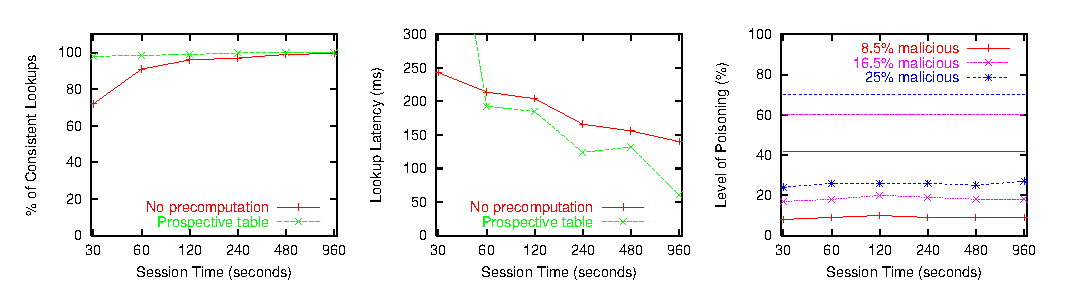
\includegraphics{results/collective.eps}}
\caption{XXX\label{fig:graphs}}
\end{figure*}

In our first experiment we measure the effects of induced churn on Bamboo. A short session time reduces Bamboo's ability to perform its proximity optimizations. Figure~\ref{fig:churn} shows that the percentage of consistent lookups increase with the peer group session time. The result confirms prior work; lower rates of churn allow routing state to stabilize. We would like to find the operating point at which Bamboo is able to stabilize and churn is able to keep malign peers at bay. 

This experiment explores whether pre-computing the routing state for the peer's next location curbs the negative effects of churn. Each peer in a group obtains a constrained routing table and leaf set from the overlay oracle prior to churning, which it uses as a seed to its next routing state. We again measure the consistency of lookups and average latencies over different session times. Figure~\ref{fig:prospect} shows that pre-computing the next routing state increases the percentage of consistent lookups. The graph also shows that the average latency is reduced since the overhead in a peer context switch is much less than the peer rejoining anew.

\subsubsection{Malicious nodes}

The following experiments introduce malicious nodes into the network. Malicious
nodes collude to mount Eclipse attacks, and thereby increase the overall level of
poisoning. A malicious node returns a reference (to itself or some malicious
colleague) in response to a routing state update message. If the malicious peer is 
unable to respond to the message (i.e., no malicious node has an identifier with the 
correct prefix) then it correctly routes the message in order to curb detection.

Figure~\ref{fig:churn_malicious} shows the level of poisoning under varying
session times. The experiment evaluates the level of poisoning when malicious 
peers make up 8.5\%,  16.5\% and 25\% of the total population. Our results 
show that churning maintains a level of poisoning around the actual fraction 
of malicious nodes. 
\eat{
\subsubsection{Diversity enforcement}
The following experiments evaluate the effects of diversity enforcement on system performance 
as well as its ability to blunt Sybil attacks. We start with the impact diversity enforcement has on 
the routing performance. A suboptimal routing table entry could be chosen because the more 
optimal entry conflicts with an already existing entry. To model this scenario, we assign the first byte of the IP address to peers through sampling IP address distributions taken from Gnutella traces~\cite{Boon}. The rest of the bits in the subnet part are filled with zeros. This simulates a worst-case scenario when all nodes that share the first byte also belong to the same subnet.  
We simulate a network of 1000 nodes with session time of 1 minute. Nodes precompute their routing tables and leafsets when moving. There are no malicious nodes. We vary the size of the subnet and measure the consistency of lookups in the presence of diversity enforcement and without. Diversity is enforced only in the routing tables and the rule used is that only a single entry belonging to a subnet is allowed in the routing table. The graphs indicate that lookups remain consistent even when a highly-restrictive diversity rule is imposed. This is due to the leafsets providing resilience to the network.
\begin{table}
\small
\caption{This table shows the percentage of routing table poisoning for different frfactions of compromised subnets where the attacker can spoof atmost 16 identities, with and without diversity.}\label{table:diversity}
\centering
\begin{tabular}{|l|l|l|}
\hline
\% of subnets &\multicolumn{2}{|c|}{\%of Routing Table poisoned}\\
\cline{2-3}
compromised&With churn&With churn and\\ 
&&diversity \\
\hline
2&20.5&11.9\\
4&35.7&24.1\\
8&46.4&39.2\\
\hline
\end{tabular}
\end{table}

In the next experiment, we test the effectiveness of diversity enforcement in preventing Sybil attacks. We vary the number of subnets that are controlled by the attacker, and study the routing table poisoning. The fraction of hosts under the attacker's control is the fraction of subnets under his control times the subnet size. If we start with a 250 node network with the attacker controlling 2\% of the subnets and the unspoofable identifier is 28 bits long, the attacker can assume 16 identities  in the subnet, and 80 in the network resulting in a magnification of his ability. We simulate a 250 node network (for which in the 16\% case has a total of 850 nodes) with 0\%, 2\%, 4\%, and 8\% compromised subnets. The attacker can spoof atmost 16 hosts. We measure the routing table poisoning. Table \ref{table:diversity} shows the effectiveness of diversity enforcement in bringing down the poisoning.
}

